\section{Method}
\begin{figure*}[t]
    \centering
    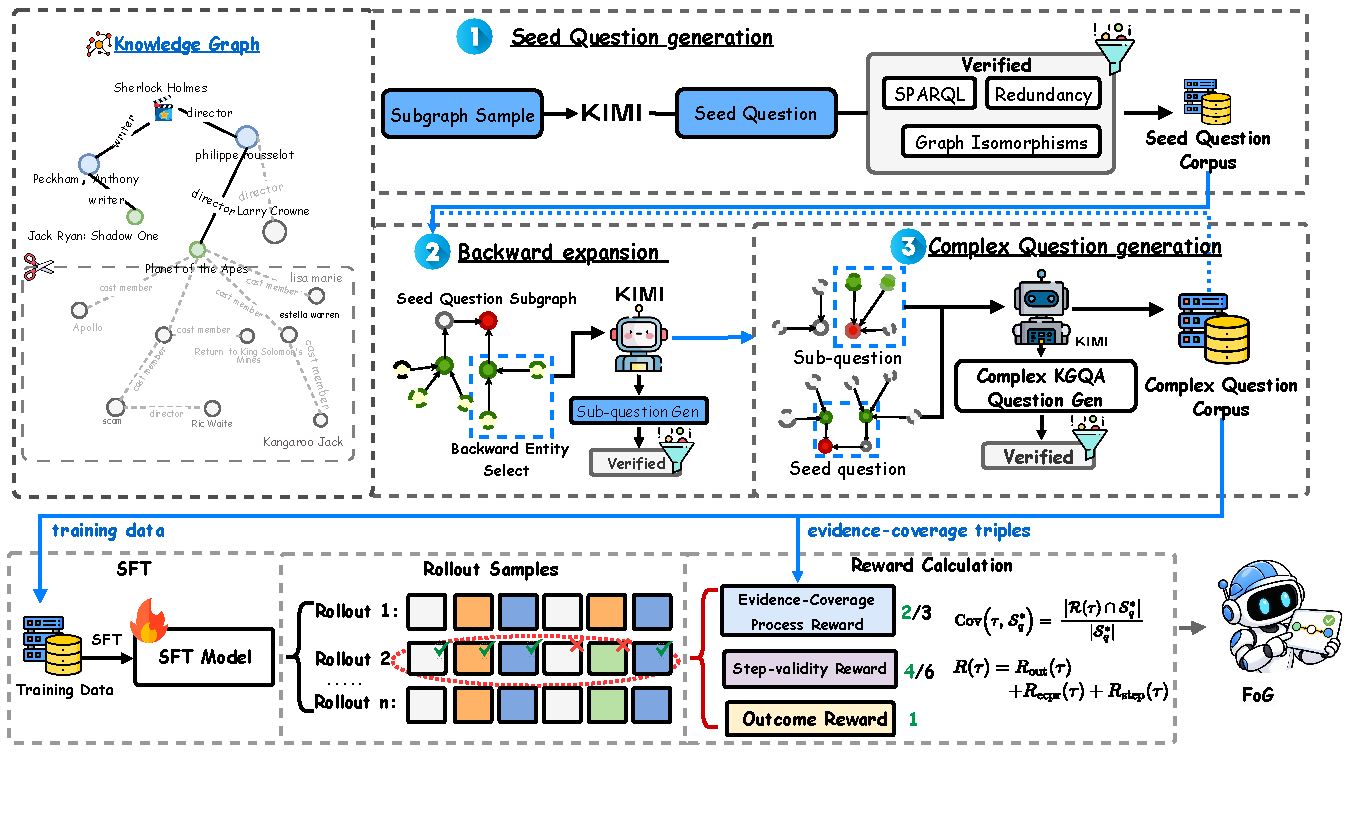
\includegraphics[width=1.0\textwidth]{figures/methods.pdf}
    \caption{\textbf{The FoG pipeline.}
    Evidence-grounded synthesis produces complex questions with gold supporting triples, the KG interaction agent records the triples that it retrieves, and ECPR rewards the retrieval of the gold supporting triples.}
    \label{fig:methods}
    \vspace{-3mm}
\end{figure*}
In this section, we introduce FoG, as shown in Figure~\ref{fig:methods}, including evidence-grounded synthesis, a KG interaction agent, and ECPR.

\noindent\textbf{Definition 1 (KG question answering).} A knowledge graph is $\mathcal{G}=(\mathcal{E},\mathcal{R},\mathcal{T})$ with entities $\mathcal{E}$, relations $\mathcal{R}$, and triples $\mathcal{T}\subseteq \mathcal{E}\times\mathcal{R}\times\mathcal{E}$. A question $q$ has a logical form $\ell_q$ and a gold answer $y_q^{*}\in\operatorname{SPARQL}(\ell_q,\mathcal{T})$, where $\operatorname{SPARQL}(\ell,\mathcal{S})$ is the result of executing $\ell$ over a triple set $\mathcal{S}$. An agent answers $q$ through a trajectory $\tau = \bigl((s_1,a_1), \ldots, (s_T,a_T)\bigr)$ of states and actions and outputs a prediction $\hat{y}$, where $\mathcal{T}_t\subseteq\mathcal{T}$ are the triples returned at step $t$, $\mathcal{T}(\tau)=\bigcup_{t}\mathcal{T}_t$ all triples retrieved along $\tau$, and $\mathcal{E}(\tau)$ all returned entities.

\noindent\textbf{Definition 2 (Supported answer).} A triple set $\mathcal{S}\subseteq\mathcal{T}$ \emph{supports} the answer of $q$ if $y_q^{*}\in\operatorname{SPARQL}(\ell_q,\mathcal{S})$. The answer of $\tau$ is \emph{correct} if $\hat{y}$ matches $y_q^{*}$, \emph{reached} if $y_q^{*}\in\mathcal{E}(\tau)$, and \emph{supported} if $\mathcal{T}(\tau)$ supports it. Unlike the first two levels, which use the KG as a source of answers, a supported answer uses it as a source of evidence. In FoG, each training question carries \emph{gold supporting triples} $\mathcal{S}^{*}_{q}$ that support its answer.

\subsection{Evidence-Grounded Synthesis}
\label{sec:synthesis}

To obtain complex questions that carry their supporting evidence, we propose evidence-grounded synthesis that includes seed question construction, backward expansion, and quality control. All roles use the teacher Kimi-K2~\citep{kimi}.

\paragraph{Seed question construction.}
We sample a size-bounded subgraph $\mathcal{G}_{\text{sub}}$ from Wikidata around a seed entity $v_{\text{seed}}$ of moderate degree. The teacher generates a 1-hop question whose answer is $v_{\text{seed}}$:
\begin{equation}
\label{eq:seed}
    \bigl(Q^{(1)}, \ell^{(1)}, \mathcal{S}^{(1)}\bigr)
    \sim \pi_{\text{gen}}\bigl(v_{\text{seed}}, \mathcal{G}_{\text{sub}}\bigr),
\end{equation}
where $\pi_{\text{gen}}$ is the teacher model, $Q^{(1)}$ the seed question, $\ell^{(1)}$ its logical form, and $\mathcal{S}^{(1)}$ its supporting triples. The seed is retained only if every triple in $\mathcal{S}^{(1)}$ exists in $\mathcal{G}_{\text{sub}}$ and $\ell^{(1)}$ executes over the global KG with $v_{\text{seed}}$ in its result set.

\paragraph{Backward expansion.}
Given a verified question $Q^{(n)}$ with logical form $\ell^{(n)}$, answer $y=v_{\text{seed}}$, and supporting triples $\mathcal{S}^{(n)}$, we replace an explicit non-answer entity $u$ in $Q^{(n)}$ with a sub-question $\tilde{Q}$ whose answer is exactly $u$:
\begin{equation}
\begin{aligned}
    &Q^{(n+1)} = Q^{(n)}[u \rightsquigarrow \tilde{Q}], \\
    &\mathcal{S}^{(n+1)} = \mathcal{S}^{(n)} \cup \tilde{\mathcal{S}}, \\
    &y \in \operatorname{SPARQL}\bigl(\ell^{(n+1)}, \mathcal{S}^{(n+1)}\bigr),
\end{aligned}
\end{equation}
where $\tilde{\mathcal{S}}$ are the supporting triples of $\tilde{Q}$, drawn from the incoming neighborhood of $u$, and $\ell^{(n+1)}$ is the expanded logical form. Each expansion turns an explicit entity into a hidden intermediate variable, and the accumulated triples still support the answer. Thus $N\in\{0,1,2\}$ expansions yield 1- to 3-hop questions, where $N=0$ keeps the seed. Expansion uses a ReAct agent~\citep{react} that retrieves the neighborhood of $u$, selects triples, writes $\tilde{Q}$, and verifies it; on failure, it reselects triples or the entity.

\noindent\textbf{Proposition 1.} \textit{Backward expansion preserves the answer and yields triples that support it.}\vspace{-2mm}
\begin{proof}\renewcommand{\qedsymbol}{}
We provide experimental results in Section~\ref{sec:rq3} and proofs in Appendix~\ref{app:proof1}.
\end{proof}

\paragraph{Quality control.}
Each synthesized question must further pass two symbolic checks, which keep the answer specific and every topic entity necessary.
\textbf{(a) Executability.} Let $\mathcal{Y}^{(n)} = \operatorname{SPARQL}(\ell^{(n)}, \mathcal{T})$ be the result set of the candidate question. We retain it only if the target answer is included and the result set is not overly broad, i.e., $y\in\mathcal{Y}^{(n)}$ and $|\mathcal{Y}^{(n)}|\le K_{\text{ans}}$ for a maximum answer-set size $K_{\text{ans}}$.
\textbf{(b) Non-redundancy.} Let $E_q$ be the topic entities of the question. We extract a shortest supporting path for each $e\in E_q$ and discard the question if a proper subset yields an equally specific answer set:
\begin{equation}
\small
\begin{aligned}
\mathcal{F}_{\mathrm{red}}(Q^{(n)})
= \mathbb{I}\!\Big[
&\exists Z \subsetneq E_q:
\mathcal{Y}^{(n)} \subseteq \mathcal{Y}^{(n)}_{Z}, \\
&|\mathcal{Y}^{(n)}_{Z}| \le |\mathcal{Y}^{(n)}|
\Big],
\end{aligned}
\end{equation}
where $\mathcal{Y}^{(n)}_{Z}$ is the answer set of the query built only from the paths of $Z$ (Appendix~\ref{app:redcheck}).

The triples accumulated for a final question $q$ are its gold supporting triples $\mathcal{S}^{*}_{q}$, and we report the distribution of query-graph types~\citep{GrailQA++} in Appendix~\ref{app:iso_dist}.

\subsection{KG Interaction Agent}
\label{sec:agent}

To make the evidence retrieved for an answer explicit, we develop a KG interaction agent that solves each question through a multi-turn think--act--observe loop with the action space
\begin{equation}
    \mathcal{A}
    =
    \{\texttt{think},\ \texttt{kg-query},\ \texttt{answer}\},
\end{equation}
where \texttt{think} performs internal reasoning, \texttt{kg-query} interacts with the KG, and \texttt{answer} emits the final prediction. The \texttt{kg-query} action is instantiated with seven atomic operations that probe the relations of an entity, expand to its neighboring entities, filter an entity set, and combine entity sets (Appendix~\ref{app:kg_ops}). Every trajectory thus records the returned triples $\mathcal{T}(\tau)$, the only evidence that FoG rewards and evaluates.

\subsection{Evidence-Coverage Process Reward}
\label{sec:training}

To train the agent to retrieve this evidence, we propose a training scheme with outcome and step-validity rewards, the evidence-coverage process reward, and turn-level policy optimization.

\paragraph{Outcome and step-validity rewards.}
We define the outcome reward of a trajectory as
\begin{equation}
\label{eq:rout}
    R_{\text{out}}(\tau)
    =
    \lambda_{\text{f1}}
    \cdot
    \operatorname{F1}(\hat{y},y_q^{*})
    +
    \lambda_{\text{ret}}
    \cdot
    \mathbb{I}[y_q^{*}\in\mathcal{E}(\tau)],
\end{equation}
where the first term rewards a correct answer and the second a reached answer. Neither term checks whether the answer is supported: a \emph{shortcut} trajectory, which outputs and even reaches the gold answer while leaving some of the supporting triples $\mathcal{S}^{*}_{q}$ unretrieved, still earns the full outcome reward.

To stabilize graph interaction, each turn also earns a step-validity reward $r^{\text{step}}_{t}=\lambda_{\text{step}}\,v_t$, where $v_t=1$ if action $a_t$ follows the required format and executes successfully, and $v_t=0$ otherwise. The trajectory-level term is the average $R_{\text{step}}(\tau)=\frac{1}{T}\sum_{t=1}^{T} r^{\text{step}}_{t}$.

\paragraph{Evidence-coverage process reward.}
Unlike the terms above, which treat the KG only as a source of answers, the \textbf{E}vidence-\textbf{C}overage \textbf{P}rocess \textbf{R}eward (ECPR) scores the trajectory against the gold supporting triples $\mathcal{S}^{*}_{q}$ provided by synthesis. We define the evidence coverage of a trajectory as
\begin{equation}
\label{eq:cov}
    \operatorname{Cov}(\tau,\mathcal{S}^{*}_{q})
    =
    \frac{
    |\mathcal{T}(\tau)\cap \mathcal{S}^{*}_{q}|
    }{
    |\mathcal{S}^{*}_{q}|
    },
\end{equation}
where $\mathcal{T}(\tau)$ are all triples retrieved along $\tau$, so a triple that the agent recalls from memory without retrieving it earns no reward. We call $\tau$ evidence-covered if $\operatorname{Cov}(\tau,\mathcal{S}^{*}_{q})=1$, and set $R_{\text{ecpr}}(\tau)=\lambda_{\text{ecpr}}\cdot\operatorname{Cov}(\tau,\mathcal{S}^{*}_{q})$. For dense credit assignment, first-match attribution assigns each gold triple to the step that first retrieves it:
\begin{equation}
    r^{\text{ecpr}}_{t}
    =
    \lambda_{\text{ecpr}}
    \cdot
    \frac{
    \bigl|(\mathcal{T}_t\cap \mathcal{S}^{*}_{q})\setminus \bigcup_{i<t}\mathcal{T}_i\bigr|
    }{
    |\mathcal{S}^{*}_{q}|
    },
\end{equation}
where $\sum_{t} r^{\text{ecpr}}_{t}=R_{\text{ecpr}}(\tau)$, so repeated retrieval of the same triple earns no additional reward. The composite reward of a trajectory is $R(\tau)=R_{\text{out}}(\tau)+R_{\text{step}}(\tau)+R_{\text{ecpr}}(\tau)$. We set $\lambda_{\text{f1}}=0.7$, $\lambda_{\text{ret}}=0.3$, $\lambda_{\text{step}}=0.5$, and $\lambda_{\text{ecpr}}=1$.

\noindent\textbf{Proposition 2.} \textit{ECPR is maximized only by supported answers and rewards each triple once.}\vspace{-2mm}
\begin{proof}\renewcommand{\qedsymbol}{}
We provide experimental results in Sections~\ref{sec:rq2} and~\ref{sec:rq5} and proofs in Appendix~\ref{app:proof2}.
\end{proof}

\paragraph{Turn-level policy optimization.}
Following prior RL-trained KG agents~\citep{Plan-Then-retrieve,KnowCoder-A1,KBQA-R1}, the policy $\pi_{\theta}$ is first initialized by supervised fine-tuning (SFT) on demonstration trajectories that a teacher model produces for the synthesized and training questions, minimizing the negative log-likelihood of the teacher actions. We then optimize it with Group Relative Policy Optimization (GRPO)~\citep{GRPO} and, following KG-R1~\citep{KG-R1}, compute the advantage per turn. For each question $q$, the policy samples $N$ trajectories $\{\tau_i\}_{i=1}^{N}$, and turn $t$ of $\tau_i$ receives the return
\begin{equation}
\label{eq:turn_return}
    G_{i,t}
    =
    R_{\text{out}}(\tau_i)
    + r^{\text{step}}_{i,t}
    + r^{\text{ecpr}}_{i,t},
\end{equation}
i.e., the shared outcome reward plus the process rewards earned by this turn. The advantage $\hat{A}_{i,t}=(G_{i,t}-\mu_q)/(\sigma_q+\delta)$ is normalized with the mean $\mu_q$ and standard deviation $\sigma_q$ of the returns over all turns of the $N$ trajectories. A turn that first retrieves gold evidence therefore receives a higher advantage than the other turns. The policy then maximizes the clipped GRPO objective with these advantages, regularized toward the SFT model (Appendix~\ref{app:advantage}).
